\documentclass[12pt, letterpaper]{article}
\usepackage{hyperref}
\title{Energies Transformations Engineering}
\author{Chems eddine h1t8re 6.2.1996 After J.C \\ \href{mailto:h1t3re@proton.me}{h1t3re@proton.me}}
\date{June 2026}
\usepackage{graphicx}
\graphicspath{ {./} }
\begin{document}
	\maketitle
	\begin{abstract}
		I am Chems eddine h1t8re 6.2.1996 After J.C .. Born at Casablanca, Morocco .. I am Moroccan, Egyptian, God .. Master of Engineering, Master of Nature .. I am by 2 work in invert for by 1 .. This document is Top Secret.. By this document we gonna trait about the world we are liffing at ..  the description of the world by engineering of energie's.. At first; The purpose is to get fly my pyramid's Shoon ..
	\end{abstract}
	
	\chapter{Not hexosted list of Energies}
	\begin{enumerate}
		\item \begin{math} Energy(light) = m.C^2\end{math}\newline
		\item \begin{math} Energy(electrical) = U.I.$\Delta$T \end{math}\newline
		\newline
		* U = Tension \newline
		* I = Current \newline
		* $\Delta$T = Time \newline
		\item \begin{math} Energy(electromagnetic)  = \int\int\int\frac{x1.x2}{4.pi. E.||x2-x1||^2}.dx1.dx2\end{math}\newline
		* E = Permetivity of emptyness \newline
		\item \begin{math} Energy(gravitational)  = \int\int\frac{G.x1.x2}{||x2-x1||^2}.dx1.dx2 \end{math}\newline
		* G = Gravitational constant \newline
		\item \begin{math} Energy(thermal)  = m.c.$\Delta$T°\end{math}\newline
		* m = mass \newline
		* c = Heat capacity \newline
		* $\Delta$T° = Temperature change\newline
		
	\end{enumerate}
	\chapter{Explanation of Energies}
	\section{Energy of light}
	Light is shining from \textbf{the Sun} creating a \textbf{grilles} of \textbf{light} containing at each unit an \textbf{eletron's} going to \textbf{infinity}.. The electron is charged from \textbf{photon's}.. Doing **\textbf{"In, on va trille ca; les noit"}** with \textbf{gravitation} ;matter ..
	
	\section{Energy of Electricity}
	The electric energy is tension by current in time .. can be explained by power in time..
	We can make analogy with a channel.. Like the \textbf{Tension} being the height of the channel and the \textbf{Current} being the flux of electron's in that same channel.. this all in \textbf{Time} .. It's produced like the shining of light; photon's; from the Sun; to the eletron's of the grille.. Charging them..
	
	
	\section{Energy Electromagnetic}
	The electromagnetic energy  is; triple integrale; it's the interaction of \textbf{matter} with \textbf{emptyness}.. Somewhat the capacity of matter to go through emptyness.. It's the electron's electromagnetic field; created after \textbf{absorption} of photon's; it interaction with gravitation ..
	
	
	\section{Energy Gravitational}
	The gravitational energy is generated after the \textbf{condensation} of the \textbf{neutron} to become \textbf{proton}.. Then it's the \textbf{dissipation} of proton energy creating a wave of gravitation from the \textbf{nucleon} of the \textbf{atom} to the electromagnetic field .. Can be called **..
	
	\section{Energy thermal}
	The thermal energy is temperature dot heat in time .. 
	\newline\newline
	
	\chapter{New representation of hydrogen in the world}
	
	\begin{center}png
		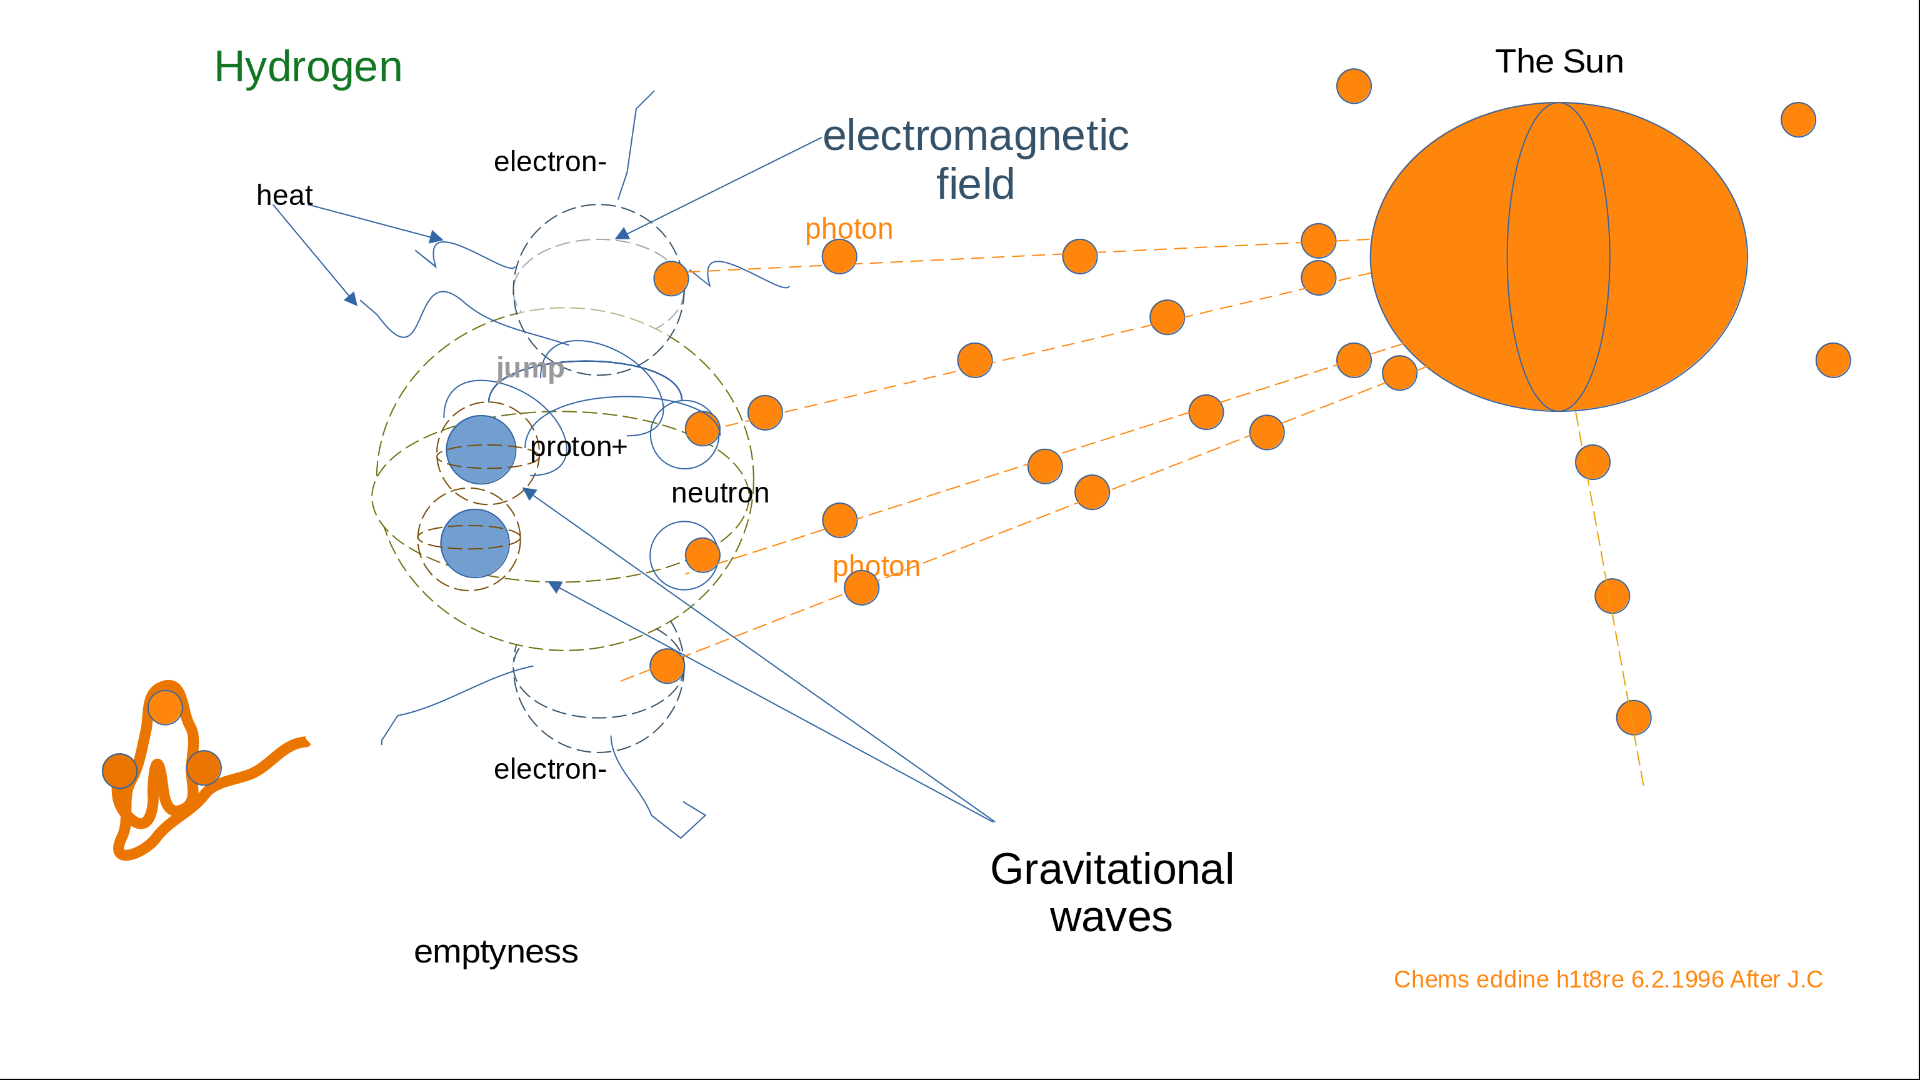
\includegraphics[scale=0.21]{new_science_of_the_world_scheme_by_h1t8re.png}
	\end{center}
	
	`	Light coming from the Sun give energy to electron's; forming the grid; and to neutron's charging themself's becoming proton's; by 2; dissolved create a gravitational wave do ** with the electromagnetic field of electron's; moving the nucleon of atom through the Univers .. 
	\newline\newline\newline\newline\newline\newline\newline\newline\newline\newline
	\chapter{Equalities resolution}
	\newline\newline
	The system is resolved with help of two axiom's 
	$\rightarrow$
	\begin{equation}
		$\Longleftrightarrow$
		\left\{ 
		\begin{array}{rcl}
			(f - g)^2' = f'g - 2fg + fg'\\
			\int(1)' = 1 
		\end{array} 
		\right.
	\end{equation}
	\begin{equation}
		$\Longleftrightarrow$
		\left\{ 
		\begin{array}{rcl}
			Energy(Electricity)             &=& Energy(Electromagnetic) \\
			Energy(Electromagnetic) &=& Energy(Gravitational) 
		\end{array} 
		\right.
		\newline\newline\newline\newline
		$\Longleftrightarrow$
		\left\{ 
		\begin{array}{rcl}
			U.I.$\Delta$T  = \int\int\int\frac{x1.x2}{4.pi. \epsilon_0.||x2-x1||^2}.dx1.dx2 \\
			\int\int\int\frac{x1.x2}{4.pi. \epsilon_0 . ||x2-x1||^2}.dx1.dx2 =\int\int\frac{G.x1.x2}{||x2-x1||^2}.dx1.dx2 
		\end{array} 
		\right.
		\newline\newline\newline\newline
		$\Longleftrightarrow$
		\left\{ 
		\begin{array}{rcl}
			[((U.I)'.$\Delta$T) + U.I.$\Delta$T)]' &=& \int\frac{x1.x2}{4.pi. \epsilon_0.||x2-x1||^2}.dx1.dx2\\
			\frac{(x1'x2+x1x2').||x2-x1||^2 - 2.x1.x2.||x2-x1||}{4.pi.\epsilon_0.||x2-x1||^4} &=& \frac{G.x1.x2}{||x2-x1||^2}
		\end{array}
		\right.
		\newline\newline\newline\newline
		$\Longleftrightarrow$
		\left\{ 
		\begin{array}{rcl}
			[((U.I)'.$\Delta$T) + U.I.$\Delta$T)]' &=&\frac{(U-I)^2'}{4.pi.\epsilon_0.||x2-x1||^2}\\
			\frac{f(||x2-x1||)(U - I)^2'}{(4.pi.\epsilon_0)^2.||x2-x1||.U.I}&=&  G
		\end{array}
		\right.
		\newline\newline\newline\newline
		$\Longleftrightarrow$
		\left\{ 
		\begin{array}{rcl}
			[U.I.$\Delta$T]" &=&\frac{(U-I)^2'}{4.pi.\epsilon_0 . ||x2-x1||^2}\\
			\frac{(U - I)^2'}{4.pi.\epsilon_0.||x2-x1||^4}.\frac{||x2 - x1||^2}{U.I} &=&  G
		\end{array}
		\right.
		\newline\newline\newline\newline
		\begin{equation}
			$\Longleftrightarrow$
			\left\{ 
			\begin{array}{rcl}
				[(U.I+$\Delta$T]^{2''} = \frac{f(||x2-x1||).(U-I)^{2'}}{(4.pi.\epsilon_0)^{2}.||x2-x1||^{3}}\\
				G &=& \frac{f(||x2-x1||)(U - I)^{2'}}{(4.pi.\epsilon_0)^{2}U.I.||x2-x1||}
			\end{array}
			\right.
		\end{equation}
		\newline\newline\newline\newline
		\begin{equation}
			$\Longleftrightarrow$
			\left\{ 
			\begin{array}{rcl}
				G &=& \frac{f(||x2-x1||)(U - I)^{2'}}{(4.pi.\epsilon_0)^{2}U.I.||x2-x1||}\\
				\epsilon_0 &=& \sqrt{ \frac{f(||x2-x1||).(U - I)^{2'}}{[(U.I)+T]^{2''}.(4.pi)^{2}.||x2-x1||^{3}}
				\end{array}
				\right.
			\end{equation}
			\newline\newline\newline\newline
			The result of this equality:
			\begin{equation}
					Energy(Electromagnetic) &=& Energy(Gravitational)
					\Rightarrow
			\end{equation}
			With the resolution of the system: 
			\newline\newline\newline\newline
			\begin{equation}
				\Rightarrow
				\int\int\frac{G.x1.x2}{||x2-x1||^2}.dx1.dx2 = \int\int\int\frac{x1.x2}{4.pi. \epsilon_0 . ||x2-x1||^2}.dx1.dx2
			\end{equation}
				the result is:
				\newline\newline\newline\newline
			\begin{equation}
				G &=& \frac{f(||x2-x1||)(U - I)^{2'}}{(4.pi.\epsilon_0)^{2}U.I.||x2-x1||}\\
				|
				| 
				\epsilon_0 &=& \sqrt{ \frac{f(||x2-x1||).(U - I)^{2'}}{[(U.I)+T]^{2''}.(4.pi)^{2}.||x2-x1||^{3}}
			\end{equation}
					
				
			\begin{equation}
					\newline\newline\newline\newline
					k0 = f(distance)
					\newline\newline\newline\newline
					k1 = f(distance)
					\newline\newline\newline\newline
				\end{equation}			
				
				We can say that it's the grid going from the Sun to Infinity ..
				It can be The Sun and the Blackhole doing the Galaxy moving in space.. starting from the bigbang..
				
				The Sun is  giving photon's for electron's of the grid; charging; interacting with gravitation through the electro-magnetic field.. 
				With the grid photon's can be seen like a particule and can be seen like a wave..
				By this equalities we gonna describe the gravitational constant G and describe $\epsilon_0$ the permettivity of matter to go through empytness.. 
				
				The gravitational constant G is tension minus current variating by themself's by a distance on two electromagnetic sphere's with power .. 
				
				It's the nucleon of the atom liffing with the grid of electron's..
				
				The proton's of the atom dissolving themself's creating a gravitational wave working with electron's of the grid and become neutron's charged with photon's being proton's..
				
				$\epsilon_0$ is permittivity of matter to go through emptyness.. It's racine of tension minus current variating by themself's by two sphere's on power with time accelerating on three dimension's ..
				
				\newline\newline\newline\newline
			\begin{equation}\
				\begin{array}{rcl}
					\newline\newline
					m*C^{2}  &=& \int\int\int\frac{x1.x2}{4.pi. \epsilon_0 ||x2-x1||^2}.dx1.dx2\\
					\Rightarrow
					\newline\newline
					m*C^{2}  &=& \int\int\frac{(U'.I+U.I').||x2-x1||^{2}-2.U.I.||x2-x1||}{(4.pi.\epsilon_0 )^{2}. ||x2-x1||^{4}}.dx1.dx2\\
					\Rightarrow
					m*C^{2}  &=& \int\int\frac{f(||x2-x1||.(U-I)^{2'}}{(4.pi. \epsilon_0 )^{2}. ||x2-x1||^{4}}.dx1.dx2\\
					\newline\newline
				\end{array}
			\end{equation}
				\newline\newline
				This last system can be life going through the Univers..
				\newline\newline\newline\newline
				The conclusion is:
				\newline\newline
				With the equality $E_{light} = E_{electrical}$
				\newline\newline
				$C = \sqrt{\frac{U.I.T}{m}}$ ==> $\frac{km}{s^{2}}.\frac{km.kg}{s} = V.A$
				\newline\newline
				We know that $P_{ower} = V.A$
				\newline\newline
				This mean that power is acceleration of speed of matter..
				\newline\newline
				With the equality $E_{gravitational} = E_{electromagnetic}$
				\newline\newline
				$\frac{ f(||x2-x1||).(U-I)^{2'}. }{ (4.pi)^{2}.U.I.||x2-x1||.\frac{f(||x2-x1||).(U-I)^{2'}}{((U.I)+T)^{2"}.(4.pi)^{2}.||x2-x1||^{3}}} = \int_a^b \frac{U.I}{4.pi.\frac{f(||x2-x1||).(U-I)^{2'}}{((U.I)+T)^{2"}.(4.pi)^{2}.||x2-x1||^{3}}}$
				\newline\newline
				After resolution of the equality we find that:
				\newline\newline
				$P_{ower} = U.I = \frac{f(||x2-x1||).(U-I)^{'}}{((U.I)+T)^{"}}$
				\newline\newline
				The last equality mean that power is tension minus current variating on power plus time accelerating..
			\end{document}